\documentclass[12pt,a4paper]{extarticle}
\usepackage[utf8]{inputenc}
\usepackage[T5]{fontenc}
\usepackage{geometry}
\geometry{a4paper, left=1.5cm, right=1cm, top=1.5cm, bottom=1.5cm, headheight=20pt, headsep=15pt, footskip=28pt}
\usepackage{enumitem}
\usepackage{multirow}
\usepackage{amssymb}
\usepackage{setspace}
\usepackage{tikz}
\usetikzlibrary{arrows.meta, positioning, calc}
\definecolor{book}{RGB}{58,90,172}
\newcommand{\noteicon}{\textcolor{book}{$\blacktriangleright$}}
\usetikzlibrary{patterns, patterns.meta, calc} % Thêm patterns.meta vào đây
% Gọi package nằm trong thư mục con template
\usepackage{../template/mngocbox}

\begin{document}
\onehalfspacing

% Sử dụng ngoặc vuông [...] để thay đổi linh hoạt các thông số
\makeheadbox[headerright={Tổng ôn 10-11},chude={CHỦ ĐỀ 08},tieude={Giới hạn và đạo hàm},dinhdang={Giải tích},lop={12 },gv={Nguyễn Lê Minh Ngọc}]

\vspace{2em}
\makeheading{I}{Tóm tắt lý thuyết}
\noindent\textbf{A. GIỚI HẠN CỦA DÃY SỐ}

\noindent\textbf{1. Giới hạn hữu hạn của dãy số}
\vspace{0.2cm}
\noindent\textit{Dãy số có giới hạn là 0}
\noindent Ta nói dãy số $(u_n)$ có giới hạn là 0 khi $n$ dần tới dương vô cực, nếu $|u_n|$ có thể nhỏ hơn một số dương bé tuỳ ý, kể từ một số hạng nào đó trở đi, kí hiệu $\lim_{n \to +\infty} u_n = 0$ hay $u_n \to 0$ khi $n \to +\infty$.
\vspace{0.2cm}

\noindent\textbf{Chú ý:} Từ định nghĩa dãy số có giới hạn 0, ta có các kết quả sau:
\begin{itemize}
    \item $\lim_{n \to +\infty} \dfrac{1}{n^k} = 0$ với $k$ là một số nguyên dương;
    \item $\lim_{n \to +\infty} q^n = 0$ nếu $|q| < 1$;
    \item Nếu $|u_n| \le v_n$ với mọi $n \ge 1$ và $\lim_{n \to +\infty} v_n = 0$ thì $\lim_{n \to +\infty} u_n = 0$.
\end{itemize}
\vspace{0.6cm}
\noindent\textit{Dãy số có giới hạn hữu hạn}

\noindent Ta nói dãy số $(u_n)$ có giới hạn là số thực $a$ khi $n$ dần tới dương vô cực nếu $\lim_{n \to +\infty} (u_n - a) = 0$, kí hiệu $\lim_{n \to +\infty} u_n = a$ hay $u_n \to a$ khi $n \to +\infty$.
\vspace{0.4cm}

\vspace{0.3cm}
\noindent\textbf{Chú ý:} Nếu $u_n = c$ ($c$ là hằng số) thì $\lim_{n \to +\infty} u_n = c$.
\vspace{0.6cm}

\noindent\textbf{2. Định lí về giới hạn hữu hạn của dãy số}

\noindent Ta có định lí về giới hạn hữu hạn của một tổng, của một hiệu, của một tích, của một thương và của một căn thức như sau:
\vspace{0.2cm}
\noindent a) Nếu $\lim u_n = a$, $\lim v_n = b$ thì:
\begin{itemize}
    \item $\lim(u_n + v_n) = a + b$;
    \item $\lim(u_n - v_n) = a - b$;
    \item $\lim(u_n \cdot v_n) = a \cdot b$;
    \item $\lim \dfrac{u_n}{v_n} = \dfrac{a}{b}$ ($v_n \ne 0, b \ne 0$).
\end{itemize}
\noindent b) Nếu $u_n \ge 0$ với mọi $n$ và $\lim u_n = a$ thì $a \ge 0$ và $\lim \sqrt{u_n} = \sqrt{a}$.
\vspace{0.4cm}

\noindent\textbf{3. Tổng của cấp số nhân lùi vô hạn}

\noindent Trong trường hợp tổng quát, ta có:
\begin{itemize}
    \item Cấp số nhân vô hạn $u_1, u_1q, \dots, u_1q^{n-1}, \dots$ có công bội $q$ thỏa mãn $|q| < 1$ được gọi là cấp số nhân lùi vô hạn.
    \item Tổng của cấp số nhân lùi vô hạn đã cho là:
    \[ S_n = u_1 + u_1q + u_1q^2 + \dots = \frac{u_1}{1 - q}. \]
\end{itemize}

\vspace{0.4cm}
\noindent\textbf{4. Giới hạn vô cực}

\noindent Ta có định nghĩa về dãy số có giới hạn vô cực như sau:
\begin{itemize}
    \item Ta nói dãy số $(u_n)$ \textit{có giới hạn} $+\infty$ khi $n \to +\infty$, nếu $u_n$ có thể lớn hơn một số dương bất kì, kể từ một số hạng nào đó trở đi.
    \item Kí hiệu $\lim_{n \to +\infty} u_n = +\infty$ hay $\lim u_n = +\infty$ hay $u_n \to +\infty$ khi $n \to +\infty$.
    \item Ta nói dãy số $(u_n)$ \textit{có giới hạn} $-\infty$ khi $n \to +\infty$ nếu $\lim_{n \to +\infty} (-u_n) = +\infty$.
    
    Kí hiệu $\lim_{n \to +\infty} u_n = -\infty$ hay $\lim u_n = -\infty$ hay $u_n \to -\infty$ khi $n \to +\infty$.
\end{itemize}
\vspace{0.4cm}
\noindent\textbf{Nhận xét:}
\begin{itemize}
    \item $\lim n^k = +\infty$ với $k$ là số nguyên dương cho trước.
    \item $\lim q^n = +\infty$ với $q > 1$ là số thực cho trước.
    \item Nếu $\lim u_n = a$ và $\lim v_n = +\infty$ (hoặc $\lim v_n = -\infty$) thì $\lim \dfrac{u_n}{v_n} = 0$.
    \item Nếu $\lim u_n = a$, $a > 0$ và $\lim v_n = 0$, $v_n > 0$ với mọi $n$ thì $\lim \dfrac{u_n}{v_n} = +\infty$.
    \item Nếu $\lim_{n \to +\infty} u_n = +\infty$ và $\lim_{n \to +\infty} v_n = a > 0$ thì $\dots \lim_{n \to +\infty} u_n v_n = +\infty$.
\end{itemize}
\vspace{0.3cm}

\noindent\textbf{B. GIỚI HẠN CỦA HÀM SỐ}

\noindent\textbf{1. Giới hạn hữu hạn của hàm số tại một điểm}
\vspace{0.2cm}

\noindent\textit{Khái niệm giới hạn tại một điểm}

\noindent Giả sử $(a; b)$ là một khoảng chứa điểm $x_0$ và hàm số $y = f(x)$ xác định trên khoảng $(a; b)$, có thể trừ điểm $x_0$. Ta nói hàm số $f(x)$ có giới hạn là số $L$ khi $x$ dần tới $x_0$ nếu với dãy số $(x_n)$ bất kì, $x_n \in (a; b), x_n \ne x_0$ và $x_n \to x_0$, ta có $f(x_n) \to L$, kí hiệu $\lim_{x \to x_0} f(x) = L$ hay $f(x) \to L$ khi $x \to x_0$.
\vspace{0.3cm}
\noindent Ta thừa nhận các định lý sau:
\noindent a) Nếu $\lim_{x \to x_0} f(x) = L$ và $\lim_{x \to x_0} g(x) = M$ ($L, M \in \mathbb{R}$) thì:
\begin{itemize}
    \item $\lim_{x \to x_0} [f(x) + g(x)] = L + M$
    \item $\lim_{x \to x_0} [f(x) - g(x)] = L - M$
    \item $\lim_{x \to x_0} [f(x) \cdot g(x)] = L \cdot M$
    \item $\lim_{x \to x_0} \dfrac{f(x)}{g(x)} = \dfrac{L}{M}$ (nếu $M \ne 0$)
\end{itemize}
\noindent b) Nếu $f(x) \ge 0$ và $\lim_{x \to x_0} f(x) = L$ thì $L \ge 0$ và $\lim_{x \to x_0} \sqrt{f(x)} = \sqrt{L}$.
\vspace{0.4cm}
\noindent\textbf{Ví dụ 5:} Tính $\lim_{x \to 0} \dfrac{\sqrt{x + 9} - 3}{x}$.
\vspace{0.6cm}

\noindent\textit{Khái niệm giới hạn một bên}
\begin{itemize}
    \item Cho hàm số $y = f(x)$ xác định trên khoảng $(x_0; b)$. Ta nói số $L$ là giới hạn bên phải của $f(x)$ khi $x \to x_0$ nếu với dãy số $(x_n)$ bất kì thoả mãn $x_0 < x_n < b$ và $x_n \to x_0$, ta có $f(x_n) \to L$, kí hiệu $\lim_{x \to x_0^+} f(x) = L$.
    \item Cho hàm số $y = f(x)$ xác định trên khoảng $(a; x_0)$. Ta nói số $L$ là giới hạn bên trái của $f(x)$ khi $x \to x_0$ nếu với dãy số $(x_n)$ bất kì thoả mãn $a < x_n < x_0$ và $x_n \to x_0$, ta có $f(x_n) \to L$, kí hiệu $\lim_{x \to x_0^-} f(x) = L$.
\end{itemize}
\vspace{0.4cm}

\noindent\textbf{2. Giới hạn hữu hạn của hàm số tại vô cực}
\vspace{0.2cm}

\noindent\textit{Khái niệm giới hạn tại vô cực}
\begin{itemize}
    \item Cho hàm số $y = f(x)$ xác định trên khoảng $(a; +\infty)$. Ta nói hàm số $f(x)$ có giới hạn là số $L$ khi $x \to +\infty$ nếu với dãy số $(x_n)$ bất kì, $x_n > a$ và $x_n \to +\infty$, ta có $f(x_n) \to L$, kí hiệu $\lim_{x \to +\infty} f(x) = L$ hay $f(x) \to L$ khi $x \to +\infty$.
    \item Cho hàm số $y = f(x)$ xác định trên khoảng $(-\infty; b)$. Ta nói hàm số $f(x)$ có giới hạn là số $L$ khi $x \to -\infty$ nếu với dãy số $(x_n)$ bất kì, $x_n < b$ và $x_n \to -\infty$, ta có $f(x_n) \to L$, kí hiệu $\lim_{x \to -\infty} f(x) = L$ hay $f(x) \to L$ khi $x \to -\infty$.
\end{itemize}
\begin{itemize}
    \item Các quy tắc tính giới hạn hữu hạn tại một điểm cũng đúng cho giới hạn hữu hạn tại vô cực.
    \item Với $c$ là hằng số, ta có: $\lim_{x \to +\infty} c = c$, $\lim_{x \to -\infty} c = c$.
    \item Với $k$ là một số nguyên dương, ta có: $\lim_{x \to +\infty} \dfrac{1}{x^k} = 0$, $\lim_{x \to -\infty} \dfrac{1}{x^k} = 0$.
\end{itemize}
\vspace{0.4cm}

\noindent\textbf{3. Giới hạn vô cực của hàm số tại một điểm}
\vspace{0.2cm}

\noindent\textit{Giới hạn vô cực}

\noindent Giả sử khoảng $(a; b)$ chứa $x_0$ và hàm số $y = f(x)$ xác định trên $(a; b) \setminus \{x_0\}$. Ta nói hàm số $f(x)$ có giới hạn $+\infty$ khi $x \to x_0$ nếu với dãy số $(x_n)$ bất kì, $x_n \in (a; b) \setminus \{x_0\}, x_n \to x_0$, ta có $f(x_n) \to +\infty$, kí hiệu $\lim_{x \to x_0} f(x) = +\infty$.
\noindent Ta nói hàm số $f(x)$ có giới hạn $-\infty$ khi $x \to x_0$, kí hiệu $\lim_{x \to x_0} f(x) = -\infty$, nếu $\lim_{x \to x_0} [-f(x)] = +\infty$.
\vspace{0.4cm}
\begin{itemize}
    \item Cho hàm số $y = f(x)$ xác định trên khoảng $(x_0; b)$. Ta nói hàm số $f(x)$ có giới hạn $+\infty$ khi $x \to x_0$ về bên phải nếu với dãy số $(x_n)$ bất kì thoả mãn $x_0 < x_n < b, x_n \to x_0$, ta có $f(x_n) \to +\infty$, kí hiệu $\lim_{x \to x_0^+} f(x) = +\infty$.
    \item Cho hàm số $y = f(x)$ xác định trên khoảng $(a; x_0)$. Ta nói hàm số $f(x)$ có giới hạn $+\infty$ khi $x \to x_0$ về bên trái nếu với dãy số $(x_n)$ bất kì thoả mãn $a < x_n < x_0, x_n \to x_0$, ta có $f(x_n) \to +\infty$, kí hiệu $\lim_{x \to x_0^-} f(x) = +\infty$.
    \item Các giới hạn một bên $\lim_{x \to x_0^+} f(x) = -\infty$ và $\lim_{x \to x_0^-} f(x) = -\infty$ được định nghĩa tương tự.
\end{itemize}
\vspace{0.4cm}
\noindent\textbf{Chú ý:} Các giới hạn $\lim_{x \to +\infty} f(x) = +\infty$, $\lim_{x \to -\infty} f(x) = +\infty$, $\lim_{x \to +\infty} f(x) = -\infty$ và $\lim_{x \to -\infty} f(x) = -\infty$ được định nghĩa tương tự như giới hạn của hàm số $f(x)$ tại vô cực. Chẳng hạn:
\noindent Ta nói hàm số $y = f(x)$, xác định trên khoảng $(a; +\infty)$, có giới hạn là $-\infty$ khi $x \to +\infty$ nếu với dãy số $(x_n)$ bất kì, $x_n > a$ và $x_n \to +\infty$, ta có $f(x_n) \to -\infty$, kí hiệu $\lim_{x \to +\infty} f(x) = -\infty$ hay $f(x) \to -\infty$ khi $x \to +\infty$. Một số giới hạn đặc biệt:
\begin{itemize}
    \item $\lim_{x \to +\infty} x^k = +\infty$ với $k$ nguyên dương;
    \item $\lim_{x \to -\infty} x^k = +\infty$ với $k$ là số chẵn;
    \item $\lim_{x \to -\infty} x^k = -\infty$ với $k$ là số lẻ.
\end{itemize}

\noindent\textbf{Một số quy tắc tính giới hạn vô cực}

\noindent Chú ý các quy tắc tính giới hạn hữu hạn không còn đúng cho giới hạn vô cực.
\noindent Ta có một số quy tắc tính giới hạn của tích và thương hai hàm số khi một trong hai hàm số đó có giới hạn vô cực.
\begin{itemize}
    \item \textit{Quy tắc tìm giới hạn của tích $f(x)g(x)$}
\end{itemize}
\noindent Giả sử $\lim_{x \to x_0} f(x) = L \ne 0$ và $\lim_{x \to x_0} g(x) = +\infty$ (hoặc $-\infty$). Khi đó $\lim_{x \to x_0} f(x)g(x)$ được tính theo quy tắc cho trong bảng sau:
\vspace{0.3cm}
\begin{center}
\renewcommand{\arraystretch}{1.3}
\begin{tabular}{|c|c|c|}
\hline
\textbf{$\lim_{x \to x_0} f(x)$} & \textbf{$\lim_{x \to x_0} g(x)$} & \textbf{$\lim_{x \to x_0} f(x)g(x)$} \\ \hline
\multirow{2}{*}{$L > 0$} & $+\infty$ & $+\infty$ \\ \cline{2-3}
& $-\infty$ & $-\infty$ \\ \hline
\multirow{2}{*}{$L < 0$} & $+\infty$ & $-\infty$ \\ \cline{2-3}
& $-\infty$ & $+\infty$ \\ \hline
\end{tabular}
\end{center}
\vspace{0.4cm}
\begin{itemize}
    \item \textit{Quy tắc tìm giới hạn của thương $\dfrac{f(x)}{g(x)}$}
\end{itemize}
\vspace{0.3cm}
\begin{center}
\renewcommand{\arraystretch}{1.3}
\begin{tabular}{|c|c|c|c|}
\hline
\textbf{$\lim_{x \to x_0} f(x)$} & \textbf{$\lim_{x \to x_0} g(x)$} & \textbf{Dấu của $g(x)$} & \textbf{$\lim_{x \to x_0} \dfrac{f(x)}{g(x)}$} \\ \hline
$L$ & $\pm\infty$ & Tuỳ ý & 0 \\ \hline
\multirow{2}{*}{$L > 0$} & \multirow{2}{*}{0} & $+$ & $+\infty$ \\ \cline{3-4}
& & $-$ & $-\infty$ \\ \hline
\multirow{2}{*}{$L < 0$} & \multirow{2}{*}{0} & $+$ & $-\infty$ \\ \cline{3-4}
& & $-$ & $+\infty$ \\ \hline
\end{tabular}
\end{center}
\vspace{0.4cm}
\noindent Các quy tắc trên vẫn đúng cho các trường hợp $x \to x_0^+$, $x \to x_0^-$.
\vspace{0.4cm}

\noindent\textbf{B. HÀM SỐ LIÊN TỤC}

\noindent\textbf{1. Hàm số liên tục tại một điểm}
\begin{itemize}
    \item Cho hàm số $y = f(x)$ xác định trên khoảng $(a; b)$ chứa điểm $x_0$. Hàm số $f(x)$ được gọi là liên tục tại điểm $x_0$ nếu $\lim_{x \to x_0} f(x) = f(x_0)$.
    \item Hàm số $f(x)$ không liên tục tại $x_0$ được gọi là gián đoạn tại điểm đó.
\end{itemize}

\vspace{0.4cm}
\noindent\textbf{2. Hàm số liên tục trên một khoảng}
\begin{itemize}
    \item Hàm số $y = f(x)$ được gọi là liên tục trên khoảng $(a; b)$ nếu nó liên tục tại mọi điểm thuộc khoảng này.
    \item Hàm số $y = f(x)$ được gọi là liên tục trên đoạn $[a; b]$ nếu nó liên tục trên khoảng $(a; b)$ và $\lim_{x \to a^+} f(x) = f(a)$, $\lim_{x \to b^-} f(x) = f(b)$.
\end{itemize}
\noindent Các khái niệm hàm số liên tục trên nửa khoảng như $(a; b], [a; +\infty), \dots$ được định nghĩa theo cách tương tự. Có thể thấy đồ thị của hàm số liên tục trên một khoảng là một đường liền trên khoảng đó.
\vspace{0.3cm}
\noindent Về tính liên tục của các hàm số sơ cấp cơ bản đã biết, ta có:
\begin{itemize}
    \item Hàm số đa thức và các hàm số $y = \sin x, y = \cos x$ liên tục trên $\mathbb{R}$.
    \item Các hàm số $y = \tan x, y = \cot x, y = \sqrt{x}$ và hàm phân thức hữu tỉ (thương của hai đa thức) liên tục trên tập xác định của chúng.
\end{itemize}
\vspace{0.4cm}

\noindent\textbf{3. Một số tính chất cơ bản}

\noindent Ta có khẳng định sau đây về tổng, hiệu, tích và thương của hai hàm số liên tục.
\vspace{0.2cm}
\noindent Giả sử hai hàm số $y = f(x)$ và $y = g(x)$ liên tục tại điểm $x_0$. Khi đó:
\begin{itemize}
    \item[a)] Các hàm số $y = f(x) + g(x)$, $y = f(x) - g(x)$ và $y = f(x)g(x)$ liên tục tại $x_0$;
    \item[b)] Hàm số $y = \dfrac{f(x)}{g(x)}$ liên tục tại $x_0$ nếu $g(x_0) \ne 0$.
\end{itemize}
\vspace{0.4cm}
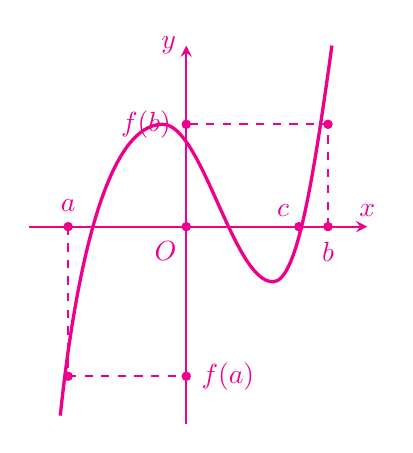
\begin{tikzpicture}[>=stealth, scale=1]
    % Định nghĩa màu magenta chủ đạo của đồ thị
    \color{magenta}
    % Hệ trục tọa độ Ox, Oy
    \draw[->, thick, magenta] (-2, 0) -- (2.3, 0) node[above] {$x$};
    \draw[->, thick, magenta] (0, -2.5) -- (0, 2.3) node[left] {$y$};
    
    % Đường cong liên tục y = f(x)
    \draw[very thick, magenta, smooth] 
        (-1.6, -2.4) .. controls (-1.4, -0.5) and (-1.0, 1.3) .. 
        (-0.3, 1.3) .. controls (0.2, 1.3) and (0.6, -0.7) .. 
        (1.1, -0.7) .. controls (1.4, -0.7) and (1.6, 0.5) .. 
        (1.85, 2.3);
    % Tọa độ các điểm chính trên đồ thị
    % P_a = (-1.5, -1.9)
    % P_b = (1.8, 1.3)
    
    % Đường gióng nét đứt (dashed) của a và f(a)
    \draw[thick, dashed, magenta] (-1.5, 0) -- (-1.5, -1.9) -- (0, -1.9);
    
    % Đường gióng nét đứt (dashed) của b và f(b)
    \draw[thick, dashed, magenta] (1.8, 0) -- (1.8, 1.3) -- (0, 1.3);
    
    % Điểm mốc trên các trục và đồ thị
    \filldraw[magenta] (0, 0) circle (1.5pt) node[below left, yshift=-2pt] {$O$};
    \filldraw[magenta] (-1.5, 0) circle (1.5pt) node[above, yshift=2pt] {$a$};
    \filldraw[magenta] (1.8, 0) circle (1.5pt) node[below, yshift=-2pt] {$b$};
    \filldraw[magenta] (1.43, 0) circle (1.5pt) node[above left] {$c$};
    
    % Điểm trên trục tung Oy
    \filldraw[magenta] (0, -1.9) circle (1.5pt) node[right, xshift=2pt] {$f(a)$};
    \filldraw[magenta] (0, 1.3) circle (1.5pt) node[left, xshift=-2pt] {$f(b)$};
    
    % Điểm giao trên đường cong
    \filldraw[magenta] (-1.5, -1.9) circle (1.5pt);
    \filldraw[magenta] (1.8, 1.3) circle (1.5pt);
    
\end{tikzpicture}

\noindent\textbf{Nhận xét:} Nếu hàm số $y = f(x)$ liên tục trên đoạn $[a; b]$ và $f(a)f(b) < 0$ thì tồn tại ít nhất một điểm $c \in (a; b)$ sao cho $f(c) = 0$.
\vspace{0.4cm}

\noindent\textbf{1. Định nghĩa đạo hàm tại một điểm}

\noindent Cho hàm số $y = f(x)$ xác định trên khoảng $(a; b)$ và $x_0 \in (a; b)$.
\noindent Nếu tồn tại giới hạn (hữu hạn) $\lim_{x \to x_0} \dfrac{f(x) - f(x_0)}{x - x_0}$ thì giới hạn đó được gọi là đạo hàm của hàm số $y = f(x)$ tại $x_0$ và kí hiệu là $f'(x_0)$ có nghĩa là:
\[ f'(x_0) = \lim_{x \to x_0} \dfrac{f(x) - f(x_0)}{x - x_0} = \lim_{\Delta x \to 0} \dfrac{\Delta y}{\Delta x} \]
\noindent Trong đó:
\begin{itemize}
    \item[] $\Delta x = x - x_0$ gọi là số gia của đối số $x$ tại $x_0$.
    \item[] $\Delta y = f(x) - f(x_0) = f(x_0 + \Delta x) - f(x_0)$ gọi là số gia tương ứng của hàm số.
\end{itemize}
\vspace{0.4cm}
\noindent\textbf{2. Đạo hàm bên trái, bên phải}
\[ f'(x_0^+) = \lim_{x \to x_0^+} \dfrac{f(x) - f(x_0)}{x - x_0}; \]
\[ f'(x_0^-) = \lim_{x \to x_0^-} \dfrac{f(x) - f(x_0)}{x - x_0}. \]
\noindent\textbf{Hệ quả:} Hàm $f(x)$ có đạo hàm tại $x_0$ khi và chỉ khi tồn tại $f'(x_0^+)$ và $f'(x_0^-)$, đồng thời $f'(x_0^+) = f'(x_0^-)$.
\vspace{0.4cm}
\noindent\textbf{3. Đạo hàm trên khoảng, trên đoạn}
\begin{itemize}
    \item[-] Hàm số $y = f(x)$ có đạo hàm trên $(a; b)$ nếu nó có đạo hàm tại mọi điểm thuộc $(a; b)$.
    \item[-] Hàm số $y = f(x)$ có đạo hàm trên $[a; b]$ nếu $f(x)$:
    \begin{itemize}
        \item[+] Có đạo hàm tại mọi $x \in (a; b)$;
        \item[+] Có đạo hàm trái $f'(b^-)$;
        \item[+] Có đạo hàm phải $f'(a^+)$.
    \end{itemize}
\end{itemize}
\vspace{0.4cm}
\noindent\textbf{4. Quan hệ giữa sự tồn tại của đạo hàm và tính liên tục của hàm số}

\noindent Nếu hàm số $y = f(x)$ có đạo hàm tại $x_0$ thì nó liên tục tại $x_0$.
\noindent\textbf{Chú ý:} Nếu $y = f(x)$ gián đoạn tại $x_0$ thì nó không có đạo hàm tại $x_0$.
\vspace{0.4cm}

\noindent\textbf{5. Ý nghĩa hình học của đạo hàm}

\noindent Đạo hàm của hàm số $y = f(x)$ tại điểm $x_0$ là hệ số góc của tiếp tuyến...

\noindent ... tuyến $M_0T$ của đồ thị hàm số tại điểm $M_0(x_0; f(x_0))$.
\vspace{0.3cm}

\noindent\textbf{Phương trình tiếp tuyến}
\noindent Phương trình tiếp tuyến của đồ thị hàm số $y = f(x)$ tại điểm $M_0(x_0; f(x_0))$ là:
\[ y - y_0 = f'(x_0)(x - x_0) \quad \text{trong đó } y_0 = f(x_0). \]
\vspace{0.3cm}
\noindent\textbf{Chú ý (tiếp):}
\begin{itemize}
    \item[+] Nếu $y = f(x)$ liên tục tại $x_0$ thì có thể không có đạo hàm tại $x_0$.
\end{itemize}
\vspace{0.4cm}
\noindent\textbf{6. Ý nghĩa vật lí của đạo hàm}
\begin{itemize}
    \item[+] Vận tốc tức thời: $v(t_0) = s'(t_0)$;
    \item[+] Gia tốc: $a(t_0) = v'(t_0) = (s'(t_0))'$;
    \item[+] Cường độ dòng điện tức thời: $I(t_0) = Q'(t_0)$.
\end{itemize}


\makeheading{II}{Bài tập tự luyện}
\noindent\textbf{1.} Tìm các giới hạn sau:
\noindent a) $\lim_{n \to +\infty} \dfrac{n^2 + n + 1}{2n^2 + 1}$;
\noindent b) $\lim_{n \to +\infty} \left(\sqrt{n^2 + 2n} - n\right)$.
\vspace{0.4cm}

\noindent\textbf{2.} Cho hai dãy số không âm $(u_n)$ và $(v_n)$ với $\lim_{n \to +\infty} u_n = 2$ và $\lim_{n \to +\infty} v_n = 3$. Tìm các giới hạn sau:
\noindent a) $\lim_{n \to +\infty} \dfrac{u_n^2}{v_n - u_n}$;
\noindent b) $\lim_{n \to +\infty} \left(\sqrt{u_n} + 2v_n\right)$.
\vspace{0.4cm}

\noindent\textbf{3.} Tìm giới hạn của các dãy số cho bởi:
\noindent a) $u_n = \dfrac{n^2 + 1}{2n - 1}$;
\noindent b) $v_n = \sqrt{2n^2 + 1} - n$.
\vspace{0.4cm}

\noindent\textbf{4.} Một bệnh nhân hàng ngày phải uống một viên thuốc $150\text{ mg}$. Sau ngày đầu, trước mỗi lần uống, hàm lượng thuốc cũ trong cơ thể vẫn còn $5\%$. Tính lượng thuốc có trong cơ thể sau khi uống viên thuốc của ngày thứ 5. Ước tính lượng thuốc trong cơ thể nếu bệnh nhân sử dụng thuốc trong một thời gian dài.
\vspace{0.4cm}

\noindent\textbf{5.} Cho tam giác $A_1 B_1 C_1$ có diện tích là 3 (đơn vị diện tích). Dựng tam giác $A_2 B_2 C_2$ bằng cách nối các trung điểm của các cạnh $B_1 C_1, C_1 A_1, A_1 B_1$. Tiếp tục quá trình này, ta có các tam giác $A_3 B_3 C_3, \dots, A_n B_n C_n, \dots$ Kí hiệu $s_n$ là diện tích của tam giác $A_n B_n C_n$.
\noindent Tính tổng $s_1 + s_2 + \dots + s_n + \dots$

\noindent\textbf{5.} Cho $f(x)$ và $g(x)$ là các hàm số liên tục tại $x = 1$. Biết $f(1) = 2$ và $\lim_{x \to 1} [2f(x) - g(x)] = 3$. Tính $g(1)$.
\vspace{0.4cm}

\noindent\textbf{6.} Xét tính liên tục của các hàm số sau trên tập xác định của chúng:
\noindent a) $f(x) = \dfrac{x}{x^2 + 5x + 6}$;
\noindent b) $f(x) = \begin{cases} 1 + x^2 & \text{nếu } x < 1 \\ 4 - x & \text{nếu } x \ge 1. \end{cases}$
\vspace{0.4cm}

\noindent\textbf{7.} Tìm giá trị của tham số $m$ để hàm số $f(x) = \begin{cases} \sin x & \text{nếu } x \ge 0 \\ -x + m & \text{nếu } x < 0 \end{cases}$ liên tục trên $\mathbb{R}$.
\vspace{0.4cm}

\noindent\textbf{8.} Tính đạo hàm của hàm số $f(x) = x^2 + 2x$ tại điểm $x_0 = 1$.

\noindent\textbf{9.} Tìm hệ số góc của tiếp tuyến của parabol $y = x^2$ tại điểm có hoành độ $x_0 = \dfrac{1}{2}$.

\makeheading{III}{Bài tập làm thêm}
\noindent\textbf{1.} Tính các giới hạn sau:
\noindent a) $\lim_{x \to 0} \dfrac{(x + 2)^2 - 4}{x}$;
\noindent b) $\lim_{x \to 0} \dfrac{\sqrt{x^2 + 9} - 3}{x^2}$.
\vspace{0.4cm}

\noindent\textbf{2.} Cho hàm số $H(t) = \begin{cases} 0 & \text{nếu } t < 0 \\ 1 & \text{nếu } t \ge 0 \end{cases}$ (hàm Heaviside, thường được dùng để mô tả việc chuyển trạng thái tắt/mở của dòng điện tại thời điểm $t = 0$).
\noindent Tính $\lim_{t \to 0^+} H(t)$ và $\lim_{t \to 0^-} H(t)$.
\vspace{0.4cm}

\noindent\textbf{3.} Tính các giới hạn một bên:
\noindent a) $\lim_{x \to 1^+} \dfrac{x - 2}{x - 1}$;
\noindent b) $\lim_{x \to 4^-} \dfrac{x^2 - x + 1}{4 - x}$.
\vspace{0.4cm}

\noindent\textbf{4.} Cho hàm số $g(x) = \dfrac{x^2 - 5x + 6}{|x - 2|}$. Tìm $\lim_{x \to 2^+} g(x)$ và $\lim_{x \to 2^-} g(x)$.
\vspace{0.4cm}

\noindent\textbf{5.} Tính các giới hạn sau:
\noindent a) $\lim_{x \to +\infty} \dfrac{1 - 2x}{\sqrt{x^2 + 1}}$;
\noindent b) $\lim_{x \to +\infty} \left(\sqrt{x^2 + x + 2} - x\right)$.
\vspace{0.4cm}

\noindent\textbf{6.} Cho hàm số $f(x) = \dfrac{2}{(x - 1)(x - 2)}$. Tìm $\lim_{x \to 2^+} f(x)$ và $\lim_{x \to 2^-} f(x)$.

\noindent\textbf{7.} Tìm $m$ để hàm số $f(x) = \begin{cases} \dfrac{x^3 - x^2 + 2x - 2}{x - 1} & \text{khi } x \ne 1 \\ 3x + m & \text{khi } x = 1 \end{cases}$ liên tục tại điểm $x = 1$.

\noindent\textbf{8.} Tìm giá trị của tham số $a$ để hàm số $f(x) = \begin{cases} \dfrac{\sqrt{x} - 1}{x - 1} & \text{khi } x > 1 \\ ax - \dfrac{1}{2} & \text{khi } x \le 1 \end{cases}$ liên tục tại điểm $x = 1$.

\noindent\textbf{9.} Cho $\lim_{x \to -\infty} \dfrac{2x + \sqrt{3x^2 - 2}}{\sqrt{4x^2 + 1} - |x|} = \dfrac{\sqrt{3} + b}{c}$. Tính giá trị của $A = b \cdot c$.


\noindent\textbf{10.} Tìm đạo hàm của hàm số $y = cx^2$ với $c$ là hằng số.

\noindent\textbf{11.} Viết phương trình tiếp tuyến của parabol $(P): y = -2x^2$ tại điểm có hoành độ $x_0 = -1$.
\end{document}